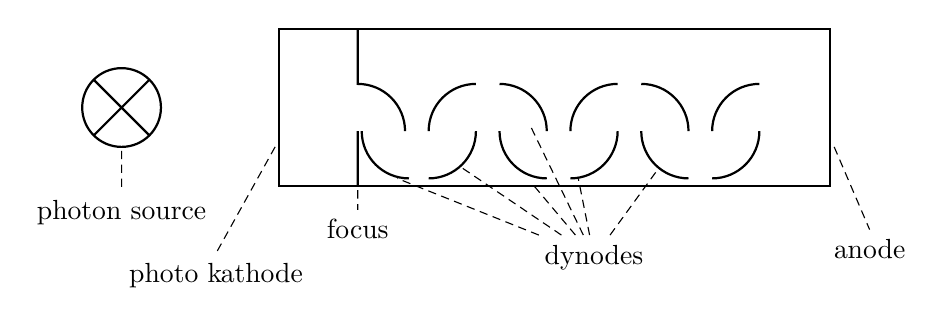
\begin{tikzpicture}
    % Röhre
    \draw[thick] (2,-1) rectangle (9,1);
    % Photonquelle
    \draw[thick]
    (0,0) circle (.5)
    (225:.5) -- (45:.5)
    (135:.5) -- (-45:.5)
    ;
    % Photokathode und Anode
    \draw[thick]
    (2,1) -- (2,-1)
    (9,1) -- (9,-1)
    ;
    % Dynoden
    \draw[thick]
    (3,-.3) -- (3,-1)
    (3,1) -- (3,.3) arc (90:0:.6cm)
    (3.05,-.3) arc (180:270:.6cm)
    (3.9,-.9) arc (270:360:.6cm)
    (3.9,-.3) arc (180:90:.6cm)
    (4.8,.3) arc (90:0:.6cm)
    (4.8,-.3) arc (180:270:.6cm)
    (5.7,-.9) arc (270:360:.6cm)
    (5.7,-.3) arc (180:90:.6cm)
    (6.6,.3) arc (90:0:.6cm)
    (6.6,-.3) arc (180:270:.6cm)
    (7.5,-.9) arc (270:360:.6cm)
    (7.5,-.3) arc (180:90:.6cm)
    ;
    % Beschriftungen PQ, PK, A und Fokussierung
    \draw[densely dashed]
    (0,-.55) -- (0,-1.05) node[below] {photon source}
    (1.95,-.5) -- (1.2,-1.85) node[below] {photo kathode}
    (3,-1.05) -- (3,-1.3) node[below] {focus}
    (9.05,-.5) -- (9.5,-1.55) node[below] {anode}
    ;
    % Beschriftung Dynoden
    \node (D) at (6,-1.9) {dynodes};
    \draw[densely dashed]
    (D) -- (3.5,-.9)
    (D) -- (4.3,-.75)
    (D) -- (5.2,-.95)
    (D) -- (5.2,-.25)
    (D) -- (5.8,-.9)
    (D) -- (6.8,-.8)
    ;
\end{tikzpicture}
